%!TEX root = ../main.tex

\chapter{Logistic Regression}
\label{chp:logistic}

\section{Introduction}
As discussed in the previous chapter, we will build a model which will predict
the outcome based on the model's learning from training dataset. Logistic Regression
is used for predicting discrete values (only 0 an 1 here) unlike continuos values in Linear Regression. It simply
calculates the probabilty of the value, calculated from Linear Regression, lying on the extremes and
output it as 0 and 1.

\section{Model} \label{sec:log_model}
The model is simply a little additional calculation on Linear Regression. We use sigmoid function
to restrict the outcome between 0 and 1. If the outcome is close to 1 then we treat it as 1 and 0 otherwise.

\subsection{Sigmoid Function}

For restricting the real number value from the outcome of Linear Regression
between 0 and 1, we use Sigmoid function. It takes real numbers as input and 
outputs continuos values between 0 and 1.

\begin{equation}
    Sigmoid(x) = \frac{1}{1+e^{-x}}
\end{equation}

The graph of Sigmoid function is shown in figure \ref{fig:sigmoid}

\begin{figure}
    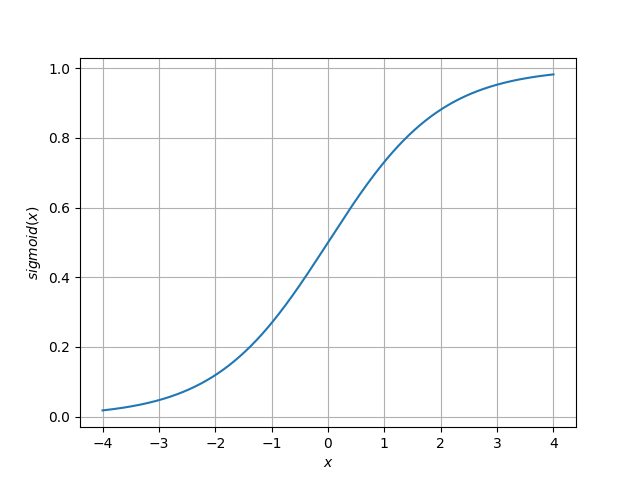
\includegraphics[]{figs/sigmoid_plot.png}
    \caption{Sigmoid function graph}
    \label{fig:sigmoid}
\end{figure}

\subsection{Mathematical Understanding}
As seen in chapter \ref{chp:linear} and discussed in section \ref{sec:log_model}, 

\begin{equation}
    y'_i = \frac{1}{1 + e^{-\vec{W} \cdot \vec{X_{(i)}}}}
\end{equation}

\subsection{Finding $W$ and $b$}
We use a little more math here to make the computation easier.
We define cost function in a slightly different way

\begin{equation}
    h_i = {(y'_i)}^{y_i}{(1-y'_i)}^{1-y_{i}}
\end{equation}

If you observe keenly and try to understand, the $h$ value gives the absolute difference between
the calculated outcome and original outcome. The original outcome is either 0 or 1. We try to spread $y'$
in such a way that the outcome of a particular instance will be close to 0 or 1 depending one
the original outcome.

As we are going to use gradient descent, we will be
calculating gradient in every round. Calculating gradient for $h$ itself is a little heavy task for computation.
We will take $\log(h)$ to make it easier.

So we will be defining the cost function as follows

\begin{equation}
    J(W,b) = \frac{1}{m} \sum_{i=1}^{m}\log{h_i}
\end{equation}

The gradient for cost function $J$

\begin{equation}
    \nabla J(W,b) = \begin{bmatrix}
        \frac{\partial J}{\partial W} \\
        \frac{\partial J}{\partial b}
    \end{bmatrix}
    = \begin{bmatrix}
        \frac{1}{m} \sum_{i=1}^{m}X^{(i)}(y_i - y'_i) \\
        \frac{1}{m} \sum_{i=1}^{m}(y_i - y'_i) 
    \end{bmatrix}
\end{equation}

Now we update $W$ and $b$ accordingly

\begin{equation}
    W_{new} = W - \alpha \frac{\partial J}{\partial W}
\end{equation}

\begin{equation}
    b_{new} = b - \alpha \frac{\partial J}{\partial b}
\end{equation}

We use the obtained $W$ and $b$ for predicting outcome. Notice here that $y'$
contains real number between 0 and 1. We will replace all the values in $y'$ greater than $0.5$
with 1 and others with 0.

\section{Questions for Curiosity}